% ### Uses XeLaTeX ### %
% ### Needs beamer-master ### %
\documentclass[aspectratio=169]{beamer} %. Aspect Ratio 16:9
\usetheme{AI2} % beamerthemeSprace.sty
% DATA FOR FOOTER
\date{2020}
\title{}
\author{}
\institute{Advanced Institute for Artificial Intelligence (AI2)}

\usetikzlibrary{calc,chains,shadows}
\usepackage{tikz}
\usepackage{subfigure}

\begin{document}    
% ####################################
% FIRST SLIDE 						:: \SliTit{<Title of the Talk>}{<Author Name>}{<Intitution>}
% SLIDE SUB-TITLE					:: \SliSubTit{<Title of the Chapter>}{<Title of the Section>}
% SLIDE WITH TITLE 					:: \SliT{<Title>}{Content}
% SLIDE NO TITLE 						:: \Sli{<Content>} 
% SLIDE DOUBLE COLUMN WITH TITLE 	:: \SliDT{<Title>}{<First Column>}{<Second Column>}
% SLIDE DOUBLE COLUMN NO TITLE 		:: \SliD{<First Column>}{<Second Column>}
% SLIDE ADVANCED WITH TITLE 			:: \SliAdvT{<Title>}{<Content>}
% SLIDE ADVANCED  NO TITLE 			:: \SliAdv{<Content>}
% SLIDE ADVANCED DOUBLE TITLE 		:: SliAdvDT{<Title>}{<First Column>}{<Second Column>}
% SLIDE ADVANCED DOUBLE NO TITLE 	:: SliAdvD{<First Column>}{<Second Column>}
% ITEMIZE 							:: \begin{itemize}  \IteOne{1st Level} \IteTwo {2nd Level} \IteThr{3rd Level} \end{itemize}
% SECTION 							:: \secx{Section} | \secxx{Sub-Section}
% COLOR BOX 						:: \blu{blue} + \red{red} + \yel{yellow} + \gre{green}
% FRAME 							:: \fra{sprace} \frab{blue} \frar{red} + \fray{yellow} + \frag{green}	
% REFERENCE						:: \refer{<doi number>}
% FIGURE 							::  \img{X}{Y}{<scale>}{Figures/.png} 
% FIGURE							:: \begin{center}\includegraphics[scale=<#>]{Figures/.png}\end{center}
% PROJECT STATUS					:: \planned\~    \started\~   \underway\~   \done\~   
% EXERCICIO							:: \Exe{<#>}{<text>}
% STACKREL							:: \underset{<down>}{<up>}
% FLUSH LEFT						:: \begin{flalign*}  & <1st equation> & \\  & <12nd equation>  & \\ \end{flalign*}
% REAL / IMAGINAY					:: \Re / \Im
% SLASH								:: \sl{} or \sl
% BOLD MATH							:: \pmb{<>}
% ####################################
%
% FIRST SLIDE :: DO NOT BREAK LINE !!!
\SliTit{Classificação}{Advanced Institute for Artificial Intelligence}{https://advancedinstitute.ai}

\SliT{Classificação}{

Agenda

\begin{itemize}
    \item O que é classificação?
    \item Classificador linear
    \item Avaliação de um classificador
\end{itemize}

}

\SliT{Classificação}{

\begin{itemize}
    \item Uma coluna na base de dados rotula cada instância da base de modo qualitativo
    \item Cada instância pode possuir dois ou mais rótulos, que são chamados de classe
    \item Um algoritmo de classificação busca descobrir para uma instância nova, a qual classe essa instância pertence, a partir de variáveis preditoras
    \item A saído do modelo pode ser também uma distribuição de probabilidade associada a cada possível classe da base de dados
\end{itemize}

}


\SliT{Classificação}{

Exemplo de classificação:

\begin{itemize}
    \item Diagnóstico médico
    \item Identificar se um atleta olímpico é halterofilista ou jogador de basquete olhando apenas sua altura e peso
    \item Detecção de fraude em cartões de crédito
    \item Filtragem de spam em e-mails
    \item Bioinformática (sequências de DNA)
\end{itemize}
}

\SliT{Classificação}{


Um conjunto de dados é separável por um modelo se :

\begin{itemize}
    \item Existe alguma instância desse aluno que prevê corretamente todos os pontos de dados 
    \item Dados separáveis linearmente 
    \item Podem separar as duas classes usando uma linha reta no espaço de características 
    \item em 2 dimensões o limite de decisão é um linha reta
\end{itemize}

}

\Sli{
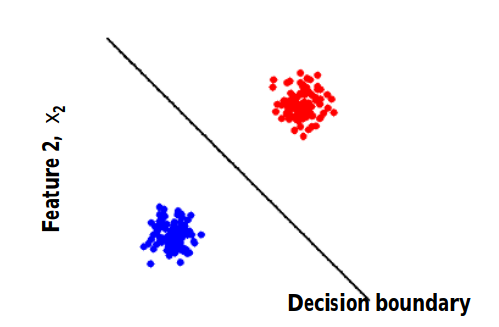
\includegraphics[width=0.45\columnwidth]{11.png}
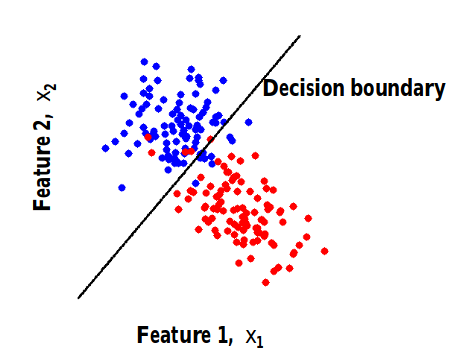
\includegraphics[width=0.45\columnwidth]{22.png}
}

\SliT{Classificação}{

Matriz de confusão 

\begin{itemize}
    \item medida efetiva do modelo de classificação
    \item mostra o número de classificações corretas versus as classificações preditas para cada classe
\end{itemize}

}

\Sli{
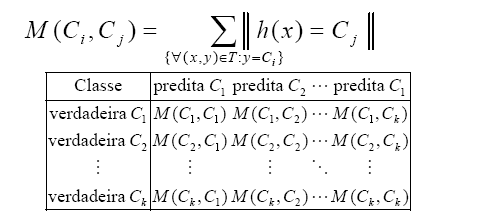
\includegraphics[width=0.65\columnwidth]{33.png}
}

\SliT{Classificação}{

\begin{itemize}
    \item O número de acertos, para cada classe, se localiza na diagonal principal M(Ci,Ci) da matriz
    \item Os demais elementos M(Ci,Cj), para i ≠ j, representam erros na classificação
    \item A matriz de confusão de um classificador ideal possui todos esses elementos iguais a zero uma vez que ele não comete erros
\end{itemize}

}


\Sli{
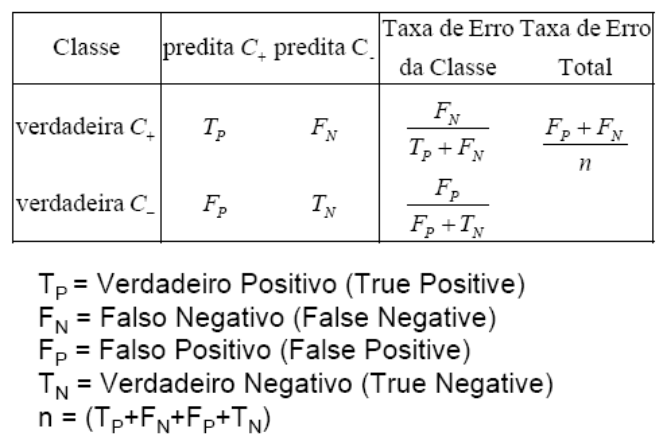
\includegraphics[width=0.55\columnwidth]{44.png}
}

\SliT{Classificação}{

Matriz de confusão 

\begin{itemize}
    \item medida efetiva do modelo de classificação
    \item mostra o número de classificações corretas versus as classificações preditas para cada classe
\end{itemize}

}

\SliT{Classificação}{
\begin{itemize}
    \item Precisão :	TP / (TP + FP)	
    \item Porcentagem de previsões positivas corretas
    \item Recall: 	TP / (TP + FN)
    \item Porcentagem de instâncias rotuladas positivamente, também previstas como   positivas
    \item Acurácia:		(TP + TN) / (TP + TN + FP + FN)
    \item Porcentagem de previsões corretas
    \item f1 score: média harmonica de precision e recall
    \item F1 score próximo de 1 indica melhor qualidade
\end{itemize}

}


\end{document}
